\section{Design Pattern}
\label{sec:design-pattern}

The design pattern used is simply using the most intuitive as possible.
The most needed are interaction and interface mockup with
With these simple and general patterns, the development process can quickly go from visualized plan into actual implementation rather than going through a long requirements document before.

% --------------------------------------------------
\subsection{Simple Interaction and Interface}
\label{ssec:simple-interfaction}

Particularly a very simple web app that doesn't require in depth logic explanation, can directly be created in a wireframe and mockup.
So that is what a simple interaction and interface can do and seen.
Wireframe is a typical way to put the bare essential elements (such as texts and images) onto a design, it contains all the information architecture.
It is a low fidelity design that shows the main software functionality without the aesthetics.
Mockup is a realistric representation to visualize the design, if we already have the information architecture that needed.
It is a middle to high fidelity design of how the software look, it basically more focus towards the aesthetics.
\autoref{fig:mockup} is an example of an already built wireframe and mockup for some part of an application.
In user's view, simple interaction and intefface can use \ac{SPA}\index{single page application} approach as the client app view.
\ac{SPA} is a web application that can fits on a one web page, so all the codes can be retrieved with only a single page load, it is a contrary to the multi page application that has many pages or windows.
In \ac{SPA}, template of the page that already is utilized to contain then present only the required data rather than sending and receiving the whole page, so that its logic can also be represented simply like in \autoref{fig:webapp}.

\begin{figure}[htbp]
    \centering
    \includegraphics[width=\textwidth]{\dir/include/wireframe-mockup.jpg}
    \caption[Wireframe vs Mockup Example]{Example of wireframe vs mockup \autocite{Trentini2015WM}}
    \label{fig:webapp}
\end{figure}

% --------------------------------------------------
\subsection{General Web App Architecture}
\label{ssec:general-webapp-arch}

General web app architecture is a non specific way to design important web application parts.
It only involves the most important parts in a web app that basically a client app for user (usually via a web browser), a server app with a database, and a protocol that connect both of them, transferring data over the network such as Internet or even a local network.
How a general web application usually architected is illustrated in \autoref{fig:webapp}.

\begin{figure}[htbp]
    \centering
    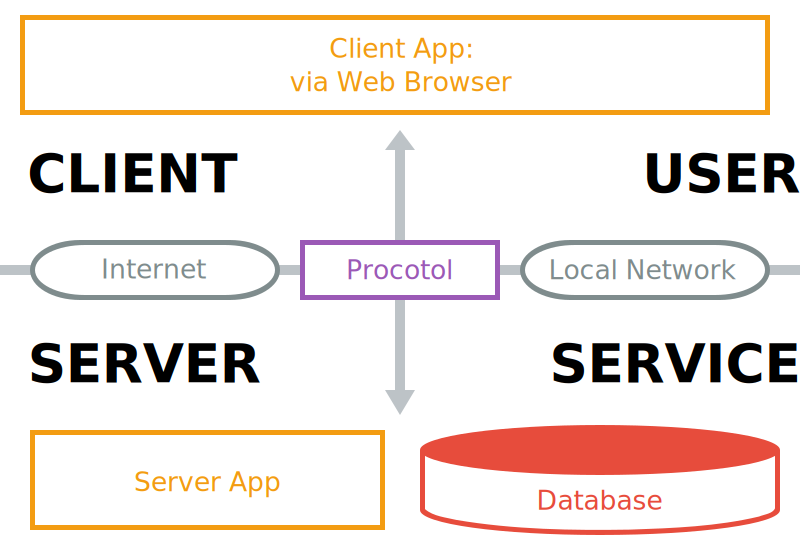
\includegraphics[width=8cm]{\dir/include/webapp.png}
    \caption[General Web Application Architecture]{Illustration of a simple general web application architecture}
    \label{fig:webapp}
\end{figure}
